
\subsection{Kullback-Leibler metoda za optimalno število stolpcev}

Naj bo $X = \{x_1, x_2, \ldots, x_n\}$ množica podatkov. Z oceno gostote verjetnosti množice $X$ z Gaussovim jedrom dobimo približek gostote verjetnosti $p$ množice $X$. Ta približek bomo primerjali s histogramom $h_n$ z n-stolpci s pomočjo Kullback-Leibler divergence po formuli:
\begin{equation}
    D_{KL}(p\|h_n) = \int_{\Omega}p(x)\cdot\log\Big(\frac{p(x)}{h_n(x)}\Big)\quad dx.
\end{equation}
Naredimo iteracijo po številu stolpcev $i = 1, \ldots, m$ za nek $m \in \mathbb{N}$. V vsaki iteraciji izračunajmo $D_{KL}(p\|h_i)$. Tisti $i$, pri katerem izraz doseže minimum, bomo vzeli za optimalno število stolpcev histograma množice $X$.

\begin{opomba}
    Zaradi zahtevnosti numeričnega računanja Kullback-Leibler divergenco v vsaki iteraciji raje računamo kot:
    \begin{equation}\label{KL-variate}
        D_{KL}(p\|h_i) = \int_\Omega p(x) \cdot ln(p(x)) dx - \int_\Omega p(x) \cdot ln(h_i(x)) dx.
    \end{equation}
    Na ta način lahko prvi člen izračunamo izven zanke, kar nam po izračunih privarčuje nekaj časa. Vemo pa tudi, da bo \eqref{KL-variate} minimalna natanko tedaj, ko bo $- \int_\Omega p(x) \cdot ln(h_i(x)) dx$.
\end{opomba}
\pagebreak
Poglejmo si, kakšne rezultate daje ta metoda v primerjavi z ostalimi.
\begin{figure}[!h]
    \centering
    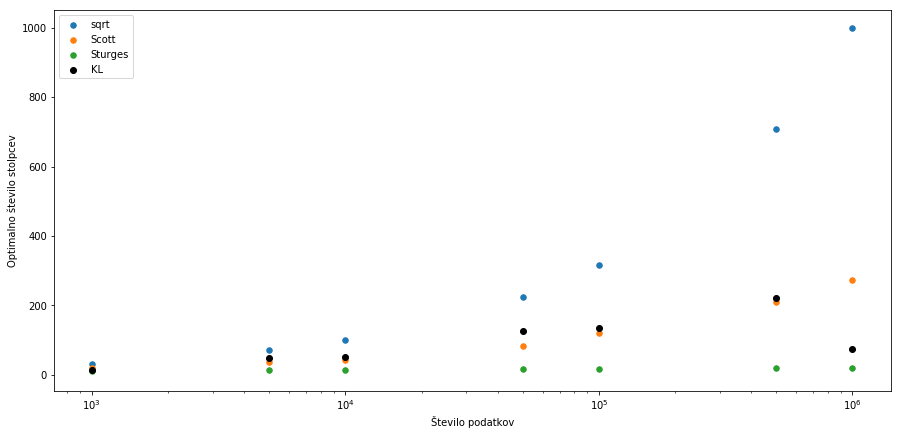
\includegraphics[width=\textwidth]{klVSostali}
    \caption{Primerjava med optimalnim številom stolpcev glede na korensko metodo in metodami Scott, Sturges in Kullback-Leibler. Os s številom podatkov je v logaritemski skali.}
\end{figure}

Zaradi preglednosti smo metodi Freedman-Diaconis in Rice izpustili. Iz slike je razvidno, da Kullback-Leibler metoda daje optimalna števila stolpcev podobna tistim, ki jih dajo ostale metode. Je pa izračun optimalnega števila stolpcev po Kullback-Leibler metodi zelo počasen, ko je število podatkov veliko. Prav tako pa procesa ne moremo optimizirati, saj funkcija $f(n) = D_{KL}(p\|h_n)$ ni konveksna, kar bi nam omogočilo iskanje minimuma, torej moramo direktno $m$-krat izračunati vrednost Kullback-Leibler divergence, kar pa je zaradi integriranja časovno zamudno.